\section{eo\-Sym\-Init$<$ Eo\-Type $>$ Class Template Reference}
\label{classeo_sym_init}\index{eoSymInit@{eoSymInit}}
Default initializer, Koza style.  


{\tt \#include $<$eo\-Sym\-Init.h$>$}

Inheritance diagram for eo\-Sym\-Init$<$ Eo\-Type $>$::\begin{figure}[H]
\begin{center}
\leavevmode
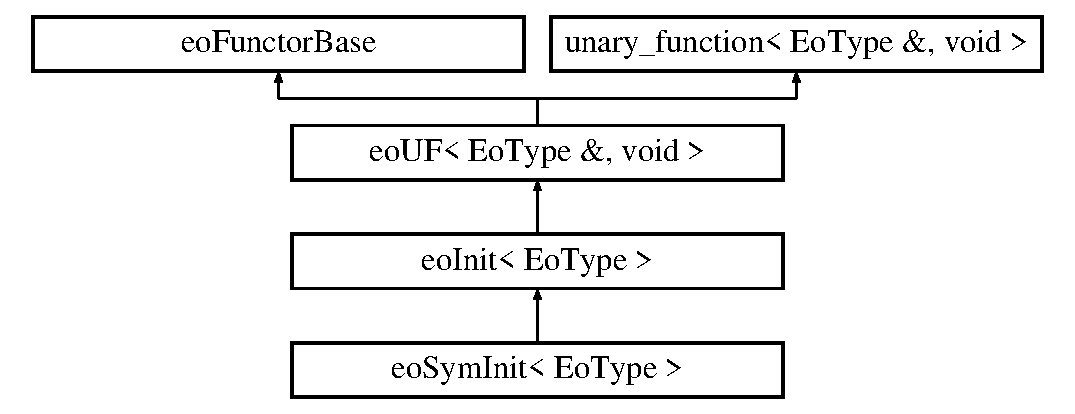
\includegraphics[height=4cm]{classeo_sym_init}
\end{center}
\end{figure}
\subsection*{Public Member Functions}
\begin{CompactItemize}
\item 
{\bf eo\-Sym\-Init} (Tree\-Builder \&\_\-builder)\label{classeo_sym_init_a0}

\begin{CompactList}\small\item\em By default build ramped half and half with max depth 6. \item\end{CompactList}\item 
{\bf eo\-Sym\-Init} (Tree\-Builder \&\_\-builder, double \&\_\-grow\_\-prob, unsigned \&\_\-max\_\-depth)\label{classeo_sym_init_a1}

\begin{CompactList}\small\item\em Control the grow\_\-prob and max\_\-depth externally. \item\end{CompactList}\item 
void {\bf operator()} ({\bf Eo\-Type} \&tree)\label{classeo_sym_init_a2}

\begin{CompactList}\small\item\em build the tree \item\end{CompactList}\end{CompactItemize}
\subsection*{Private Attributes}
\begin{CompactItemize}
\item 
Tree\-Builder \& {\bf builder}\label{classeo_sym_init_r0}

\item 
double {\bf own\_\-grow\_\-prob}\label{classeo_sym_init_r1}

\item 
unsigned {\bf own\_\-max\_\-depth}\label{classeo_sym_init_r2}

\item 
double \& {\bf grow\_\-prob}\label{classeo_sym_init_r3}

\item 
unsigned \& {\bf max\_\-depth}\label{classeo_sym_init_r4}

\end{CompactItemize}


\subsection{Detailed Description}
\subsubsection*{template$<$class Eo\-Type$>$ class eo\-Sym\-Init$<$ Eo\-Type $>$}

Default initializer, Koza style. 



Definition at line 26 of file eo\-Sym\-Init.h.

The documentation for this class was generated from the following file:\begin{CompactItemize}
\item 
eo\-Sym\-Init.h\end{CompactItemize}
